\section{\SYSTEM{}: Learning Control}
\label{sec:framework}


\PUNT{To do so, we must quickly build a model of the new application
  and then control its resource usage such that it meets a desired
  performance target with minimal energy.}

\begin{figure}
  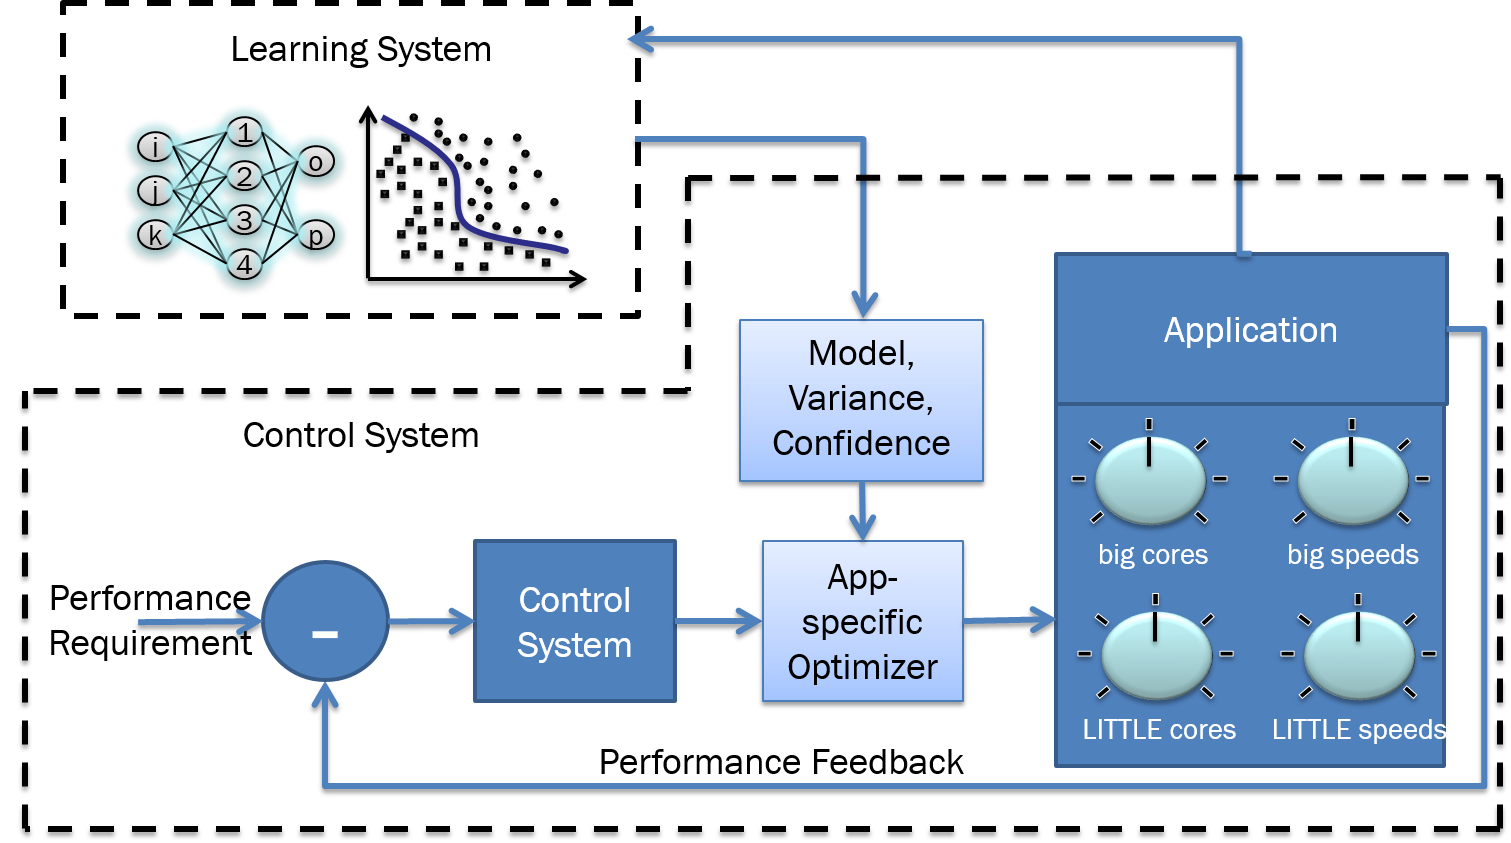
\includegraphics[width=\columnwidth]{figures/Overview.png}
  \caption{\SYSTEM{} overview.}
  \label{fig:overview}
\end{figure}


We describe \SYSTEM{}'s parmeter-free resource management system,
which assumes no prior knowledge of the application and requires no
user-specified parameters.  \figref{fig:overview} shows \SYSTEM{}'s
approach to this problem.  A generalized adaptive control system (GCS)
allocates resources to the new application to meet its specified
performance goal with minimal energy.  The GCS starts with a generic
resource model, allocates resources according to that model, and
records performance and power for a small number of configurations.
The recorded values are sent to a learning system, which estimates the
application's performance and power in all other configurations and
extracts those that represent Pareto-optimal tradeoffs in
performance/power.  These configurations are packaged in a special
data structure---the performance hash table (PHT).  The learner sends
the PHT, the estimated variance, and a confidence interval to the
control system.  Using these values, the GCS selects an energy minimal
resource configuration in constant time with formal guarnatees that it
will converge to the desired performance.

\begin{figure}
  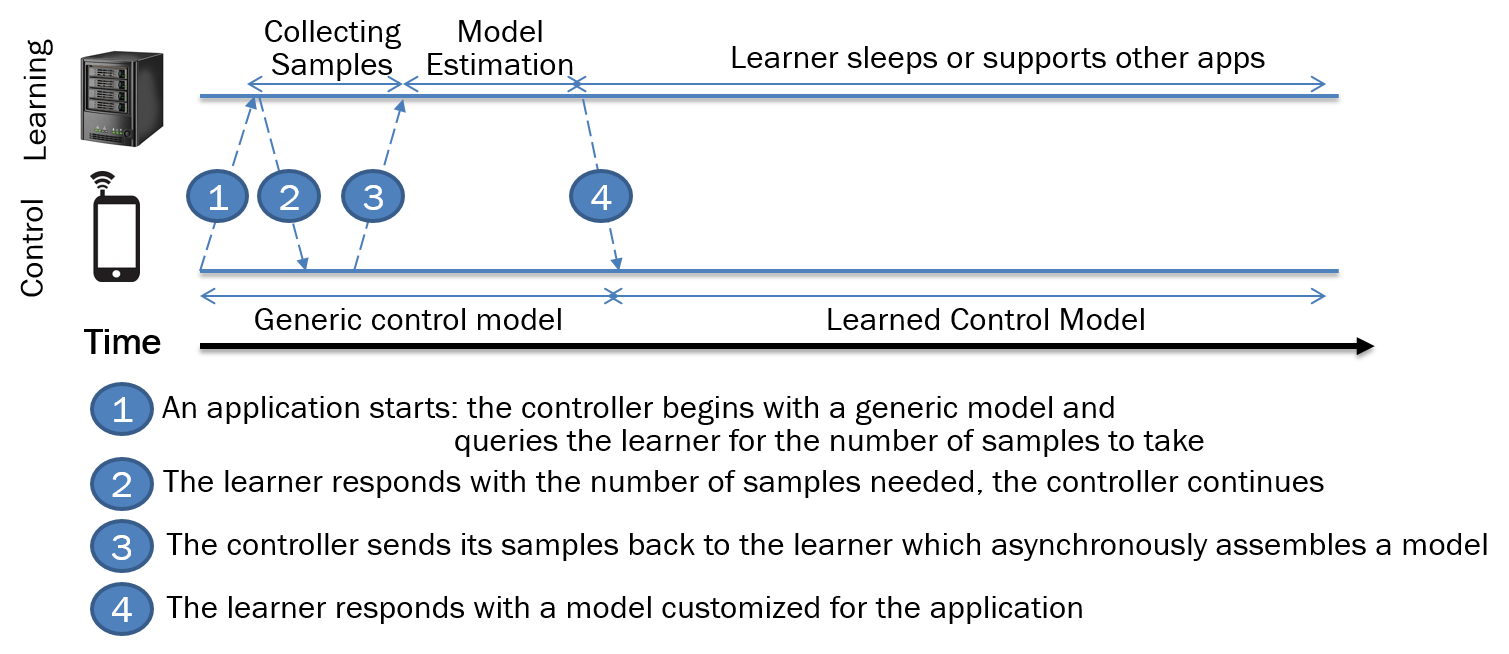
\includegraphics[width=\columnwidth]{figures/Timeline.png}
  \caption{Temporal relationship of the learning and control system.}
  \label{fig:timeline}
\end{figure}

\figref{fig:timeline} illustrates the asynchronous interaction between
\SYSTEM{}'s learning and control systems over time. The controller
starts when a new application launches with a performance goal.  Since
the controller has no prior knowledge of this application it starts
with a generic system model and allocates resources to the application
using this model.  At application launch, the controller sends a
message to the learner (message 1, in the figure) specifying the
application name and device type.  Based on the application and
device, the learner determines how many samples it needs for an
accurate estimate and sends this back to the controller (message 2).
The controller takes these samples during the course of applying the
generic model to determine resource configurations.  Once the correct
number of samples are measured, the controller sends the learner a
message with the performance and power of each measured configuration
(message 3).  Computationally expensive learners may require some time
to build a model from these observations.  Once the learner has a
model and variance estimate, that data is sent back to the controller
(message 4). From that point on, the controller uses this learned model.  

\figref{fig:timeline} shows several key points about the relationship
between learning and control.  First, the controller never waits for
the learner---it uses a generic model to provide less efficient
control until the learner can produce a customized model. Second, the
controller does not need to conintuously communicate with the learner,
this interaction happens once at application launch.  Third, if the
learner crashed, the controller would just default to the behavior of
a generic adaptive control system.  If the learner crashed after
producing a model, the control might not even need to know.  Finally,
because the learner and controller have a clearly defined interface,
they can be run in separate processes or even on physically separate
devices.

In the remainder of this section, we first describe a typical adaptive
control system would look like if designed for a heterogeneous
processor.  We then describe how we generalize this approach and
separate out parameters to be learned.  Next, we describe the general
class of learning systems that can work with this approach.  Then, we
describe how to encode the learned model so that it can be efficiently
accessed by the controller.  Finally, we discuss the formal guarantees
provided by the \SYSTEM{} approach.


\subsection{Traditional Control for Computing}
Several researchers have proposed techniques for controlling computing
systems.  A controller that can manage multiple resources to meet
multiple goals is known as a multiple-input, multiple-ouput (MIMO)
controller.  The inputs are measurements, \eg{} performance.  The
outputs are the resource settings to be used at a particular time,
\eg{} an allocation of big and LITTLE cores and a clockspeed for each.

The following difference equations describe a generic MIMO controller
for allocating $n$ resources to meet $m$ goals at time
$t$:\footnote{We assume discrete time, and thus, use diffference
  equations rather than differential equations that would be used for
  continuous systems.}
\begin{equation}
\begin{aligned}
&\x(t+1) &=& \mathbf{A} \cdot \x(t)& + \mathbf{B} \cdot \mathbf{c}(t)\\
&\y(t)   &=& \mathbf{C} \cdot \x(t)&
\end{aligned}
\label{eqn:system:mimo}
\end{equation}
Where $\x \in \R^{q}$ is the controller's \emph{state}, an abstract
representation of the relationship between resources.  $\mathbf{c}(t)
\in \R^n$ is a vector representing the current \emph{configuration} of
resources; \ie{} the $i$th vector element represents the amount of
resource $i$ to be allocated at time $t$.  $\y(t) \in \R^{m}$
represents the current value of the goal dimensions at time $t$. The
matrices $\mathbf{A} \in \R^{q \times n}$ and $\mathbf{B} \in \R{q
\times n}$ relate the resource configuration to the controller state.
The matrix $\mathbf{C}$ relates the controller state to the expected
behavior.  This model does not assume the states or the resources are
independent, but it does assume that their relationship is linear.  

For example, to allocate resources to meet performance goals in our
ARM big.LITTLE system---from \secref{example}---there are four
resources: the number of big cores, the number of LITTLE cores, and
the speeds for each of the big and LITTLE cores.  There is also a
single goal: performance.  Thus, in this example, $n=4$ and $m=1$.
The matrices $\mathbf{A}$, $\mathbf{B}$, and $\mathbf{C}$.  In this
example, we know there is a non-linear relationship between the
resources.  We can overcome this difficulty by tuning the identified
matrices at each time step---approximating the non-linear system
through a series of changing linear formulations.  This approximation
is a form of \emph{adaptive} or \emph{self-tuning} control
\cite{adaptiveControl}.  Such adaptive controllers provide formal
guarantees that they will converge to the desired performance even in
the face of non-linearities, but they still assume convexity.

This control formulation has several drawbacks.  First, because it
requires matrix computation, its overhead scales linearly in the
number of resources \cite{Hellerstein2004a,METE}.  Second, the
adaptive mechanisms are not parameter-free---they require starting
values of the matrices $\mathbf{A}$, $\mathbf{B}$, and
$\mathbf{C}$---these inital values must be provided by the user and
they must account for non-linearity in the relationship between
resources \cite{POET,METE,AdaptiveControl}.  Therefore, typically 100s
to 1000s of samples are taken before the controller is designed to
ensure that the starting matrices are sufficient to prevent the
controller from getting stuck in a local optima \cite{FSE2015,sysid}.
Finally, these techniques cannot minimize energy.  While
\emph{optimal} control techniques exist, they find the minimal change
in resources that can meet the goal; \ie{} they cannot minimize some
other function of the resources, like energy consumption
\cite{josep-isca2016,Hellerstein2004a,optimal-control}.

\subsection{\SYSTEM{} Control System}
To overcome the above issues, \SYSTEM{} abstracts the controller of
\eqnref{system:mimo} and factors out those parameter that can be
estimated by a learner.  Specifically, \SYSTEM{} takes three steps to
transform a standard control system into one that can allocate
resources to meet a performance goal with minimal energy.  The first
step is controlling \emph{speedup} rather than directly controlling
resources.  The second step is to translate speedup into an energy
minimal \emph{resource schedule}.  The third step is to exploit the
structure of this scheduling problem so that it can be solved in
constant time, assuming a separate learner has produced a model of
resource performance and power.  The result is that \SYSTEM{}'s
controller runs in constant time without requiring any user-specified
parameters.

% We first describe our formulation for controlling speedup and then
% converting that speedup into resource allocations.

\subsubsection{Controlling Speedup}
Instead of the matrix equations of \eqnref{system:mimo}, \SYSTEM{}
uses a scalar difference model relating speedup to performance:
\begin{equation}
  perf(t) = b \cdot speedup(t-1) + \delta \label{eqn:speedup}
\end{equation}
where $b$ is the application's \emph{base speed}: defined as the speed
when all resources are available.  While $b$ is application specific,
it is easy to measure online, by simply allocating all resources. Such
a configuration should not violate any performance constraints
(although it is unlikely to be energy efficient) so it is safe to take
this measurement.

With this model, \SYSTEM{}'s control law is simply:
\begin{eqnarray}
  error(t) &=& goal - perf(t) \label{eqn:speedup-error} \\
  speedup(t) &=& speedup(t-1) - \frac{error(t)}{b}
  \label{eqn:speedup-control}
\end{eqnarray}
which states that the speedup at time $t$ is a function of the
previous speedup, the error at time $t$ and the base speed.  This is a
very simple \emph{deadbeat} controller that provides all the standard
control theoretic formal guarantees \cite{ControlHandbook}.

By measuring base speed online while the application runs, we tune the
controller to a specific application; using this definition of base
speed, most speedups will be less than one.  We can further generalize
\eqref{eqn:speedup-control} as:
\begin{equation}
speedup(t) = speedup(t-1) - \frac{1 - \rho(t)}{b}.error(t)
\end{equation}
where $0 \le \rho(t) < 1$ is a pole of the controller's characteristic
equation.  At small values of $\rho(t)$ the controller will eliminate
error quickly, but may overreact to noise or model inaccuracies.
Larger $\rho(t)$ makes the system more robust at the cost of reduced
convergence time.  \emph{Dynamically setting the pole to account for
  error in the learned models will be a key of combining control and
  learning.}  First, however, we address the challenging problem of
converting an abstract speedup into an actual resource allocation.

\subsubsection{Converting Speedup to Resource Allocation}
\SYSTEM{} must map \eqnref{speedup-control}'s speedup into a resource
allocation.  On our example ARM big.LITTLE architecture that
specifically means mapping speedup into an allocation of big and
LITTLE cores as well as a speed for both (big and LITTLE cores are in
separate clock domains).

The primary challenge is that speedups and powerups in real systems are a discrete non-linear
function of resource usage, while
\eqnref{speedup-control} is a continuous linear function.  We bridge
this divide by assigning time to resource allocations such that the
average speedup over a control interval is that produced by
\eqnref{speedup-control}.

We call an assignment of time to resources a schedule. There are
typically many schedules that meet a particular performance
requirement and we want to find a minimal energy schedule. Given a
time interval $T$, a speedup requirement $speedup(t)$ to average over
the time interval, and a configuration set of size $C$ , we formalize
this problem as:
\begin{eqnarray}
  \minimize_{\mathbf{\tau} \in \R^{C}} && \sum_{c=0}^{C-1} \tau_c \cdot p_c \label{eqn:power}  \\
  \st %&& \nonumber\\
  && \sum_{c=0}^{C-1} \tau_c \cdot s_c =  speedup(t)T \label{eqn:work} \\
  && \sum_{c=0}^{C-1} \tau_c =  T \label{eqn:deadline} \\
  && 0 \le \tau_c \le T, \qquad \forall c \in \{0,\ldots,C-1\} \label{eqn:time}
\end{eqnarray}
where $p_c$ and $s_c$ are configuration $c$'s estimated powerup and
speedup; $\tau_c$ is the time to spend in configuration $c$.
\eqnref{power} simply states that the objective is to minimize energy
(power times time).  \eqnref{work} states that the average speedup
must be maintained, while \eqnref{deadline} requires the time to be
fully utilized.  \eqnref{time} simply avoids negative time.


\subsection[Learning Power/Performance Tradeoffs]{Hierarchical Bayesian Models}
\PUNT{
\begin{figure}
\centering
  \subfloat[]
  {
    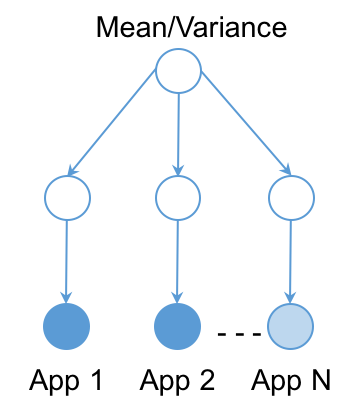
\includegraphics[width=.2\textwidth]{figures/HBM.png}
  }
  \caption{ A Hierarchical Bayesian model.  The arrows represent
    dependences, circles are random variables, white circles are
    hidden variables that cannot be observed and must be learned,
    solid circles represent fully observed data, and shaded circles
    represent partially observed data.}
\label{fig:learning-models}
\end{figure}

\begin{figure*}

  \subfloat[]
  {
    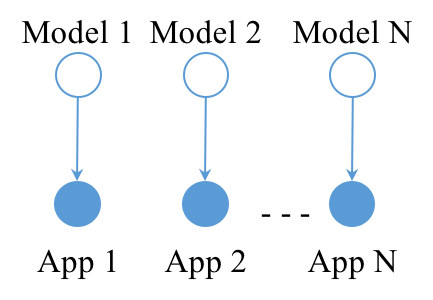
\includegraphics[width=.33\textwidth]{figures/Online.png}
    \label{fig:online}
  }
  \subfloat[]
  {
    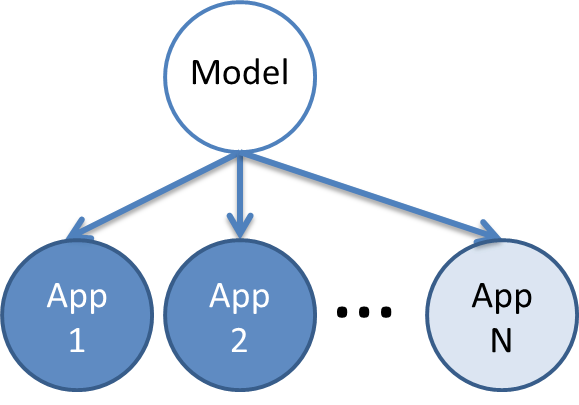
\includegraphics[width=.33\textwidth]{figures/Offline.png}
    \label{fig:offline}
  }
  \subfloat[]
  {
    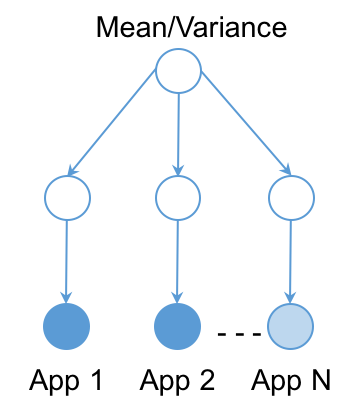
\includegraphics[width=.33\textwidth]{figures/HBM.png}
    \label{fig:HBM}
  }
  \caption{ Comparison of online (a) offline (b) and hierarchical
    Bayesian models (c).  The arrows represent dependences, circles
    are random variables, white circles are hidden variables that
    cannot be observed and must be learned, solid circles represent
    fully observed data, and shaded circles represent partially
    observed data.  The online model is concerned only with the
    current application (labeled N), the offline model combines all
    observations into one model, and the HBM builds per-application
    models, but makes them conditionally dependent on one another so
    that prior observations can be used to increase the accuracy of
    the model built for application N.}
\label{fig:learning-models}
\end{figure*}
}

Assuming no prior knowledge of the application, we estimate its power
($p_c$) and performance ($s_c$) in configuration $c$.
\PUNT{Specifically, we take observations of performance and power in a
  resource configuration and predict (1) how future applications will
  perform or (2) how different resource allocations affect the current
  application.}  \SYSTEM{} uses a hierarchical Bayesian model (HBM) to
turn observations of an application's performance and power into
predictions about how other, unobserved resource allocations will
affect performance and power.  The HBM provides a statistically sound
framework for learning across applications and devices; \ie{} it
handles the non-convex tradeoff spaces heterogeneity produces (\eg{}
\figref{fig:lavamd_contour}).

The HBM provides balance between completely online approaches -- which
consider only the current application -- and offline approaches --
which consider only prior applications approaches.  \PUNT{ Each
  application has its own model, allowing specificity, but these
  models are conditionally dependent on some underlying probability
  distribution with a hidden mean and co-variance matrix.  In
  practice, the HBM will estimate a model for a new application using
  a small number of observations and combining those observations with
  the large number of observations previously made of similar
  applications.  Rather than over-generalizing, the HBM will use only
  similar applications to learn models.  In addition, the HBM's
  accuracy increases as more applications are observed because more
  different types of behavior are represented in the pool of prior
  knowledge.  Of course, the computational complexity of learning also
  increases with increasing applications, but this is why we offload
  the learning to a remote server.  } Consider a simplified example.
Suppose we have observed many prior applications, all of which are
either completely compute-bound or completely memory-bound, and we
have an equal number of both.  The only resource we can allocate is
clockspeed, which will increase the performance of compute-bound
applications, but not memory-bound ones.  When we need to work with a
new application, we need to estimate its response to clockspeed.  The
online model does not use prior knowledge, but will observe many
different clock speeds for the new application, leading to high
overhead.  A fully offline model predicts the mean response of prior
applications, meaning it will over-allocate speed to memory-bound
applications and under-allocate to compute-bound ones.  The HBM takes
a small number of observations and combines those with prior
knowledge: if the new observations show that clockspeed has no effect
on performance the HBM will use only the prior memory bound
applications to build its model, otherwise, it will use the
compute-bound applications.  In practice, the HBM can learn much more
complicated tradeoffs by combining observations of the new application
with prior knowledge of different types of behavior.

\PUNT{
When selecting a learning framework we must find a tradeoff between
the specific and the general; \ie{} between frameworks that build
application-specific models and frameworks that combine observations
across applications.  For example, the key to energy efficiency on
heterogeneous mobile systems is knowing when to make use of the
smaller, low-power cores \cite{}.  An application-specific model will
capture that precisely, but may require many observations before
producing the correct model.  A more general model will capture the
trend, \eg when most applications should transition, but this general
model might miss the key inflection point for some applications.  We
refer to application-specific models as \emph{online} because they
build models for the current application and do not incorporate
knowledge of other applications.  We refer to general models as
\emph{offline} as they use prior observations of other applications to
predict the behavior of a new application.
}

Now we describe our HBM model in details. Suppose our system has $n = |\mathcal{C}|$ configurations and we have a set of $m-1$
applications whose performance and power are known (\ie{} they have
been measured offline). Let the vector $\y_i \in \R^{n}$ represent
application $i$'s performance (or power) estimate in all $n$
configurations; \ie{} the $c$th component of $\y_i$ is the performance for
application $i$ in configuration $c$ (or $\y_i[c] = p_c$).  Also, let
$\{\y_i\}_{i =1}^m$ be shorthand for the performance estimates of all
applications.  Without loss of generality, we assume the first $m-1$
columns, \ie{} $\{\y_i\}_{i =1}^{m-1}$ represent the data for those
applications whose performance measurement is collected offline.  The $m$th
column, $\y_m$ represents the performance measurement for the new, unknown
application.  We have a few observations for this application.
Specifically, for the $m$th application we have observed
configurations belonging to the set $\Omega_m$ where $|\Omega_m| \ll
n$.  The HBM estimates application $m$'s performance for all unobserved
configurations using the following statistical model:
\begin{equation}
\begin{aligned}
\y_i \vert \z_i  &\sim N( \z_i, \sigma^2 \I),\\
\z_i \vert \mu,\Sigma &\sim N(\mu, \Sigma),\\
\mu, \Sigma &\sim N(\mu_0,\Sigma / \pi)IW(\Sigma | \nu, \Psi),
\end{aligned}
\label{eq:HBN}
\end{equation}

where $\y_i \in \R^n, \; \z_i \in \R^n, \; \mu \in \R^{n}, \; \Sigma
\in \R^{n\times n}$. In this model the performance (denoted by $\y_i$) of
the $i^{th}$ application, is drawn from multivariate-Gaussian
distribution with mean $\z_i$ and a diagonal covariance matrix
$\sigma^2\I$.  Similarly, $\z_i$ is from multi\-variate-Gaussian
distribution with mean $\mu$ and covariance $\Sigma$. And, $\mu$ and
$\Sigma$ are jointly drawn from normal-inverse-Wishart distribution
with parameters $\mu_0, \pi,\Psi, \nu$.  Our model's parameters are
$\mu,\Sigma$, whereas, $\mu_0, \pi,\Psi, \nu$ are the
hyper-para\-meters, which we set as $\mu_0 = 0, \pi = 1,\Psi = \I, \nu =
1$.  We solve the above equations using an
\emph{estimation-maximization} algorithm to get a value of $\z_M$,
which serves as an estimator for the target application.




\subsection{Encoding Learned Models}
Given the HBM's estimates of speedup and power, we now need to solve
\eqnrref{power}{time}.  The GCS solves this on the local device, so
solution must be found efficiently.  To achieve this efficiency we (1)
exploit the structure of this particular optimization and (2) encode
the HBM's model in a performance hash table (PHT).  Combining these
two ideas we solve \eqnrref{power}{time} in constant ($O(1)$) time.

Kim et al. analyze solutions to the problem of minimizing
energy while meeting a performance constraint \cite{kim-cpsna}.  They
observe that there must be an optimal solution with the following
properties:
\begin{itemize}
\item At most two of $\tau_c$ are non-zero, meaning that at most two
  configurations will be used in any time interval.
\item If you chart the configurations in the power and performance
  tradeoff space the two configurations with non-zero $\tau_c$ lie on
  the lower convex hull of the power performance tradeoff space.
\end{itemize}
We use these two facts to construct a constant time algorithm for
finding the optimal solution online.

\begin{figure}
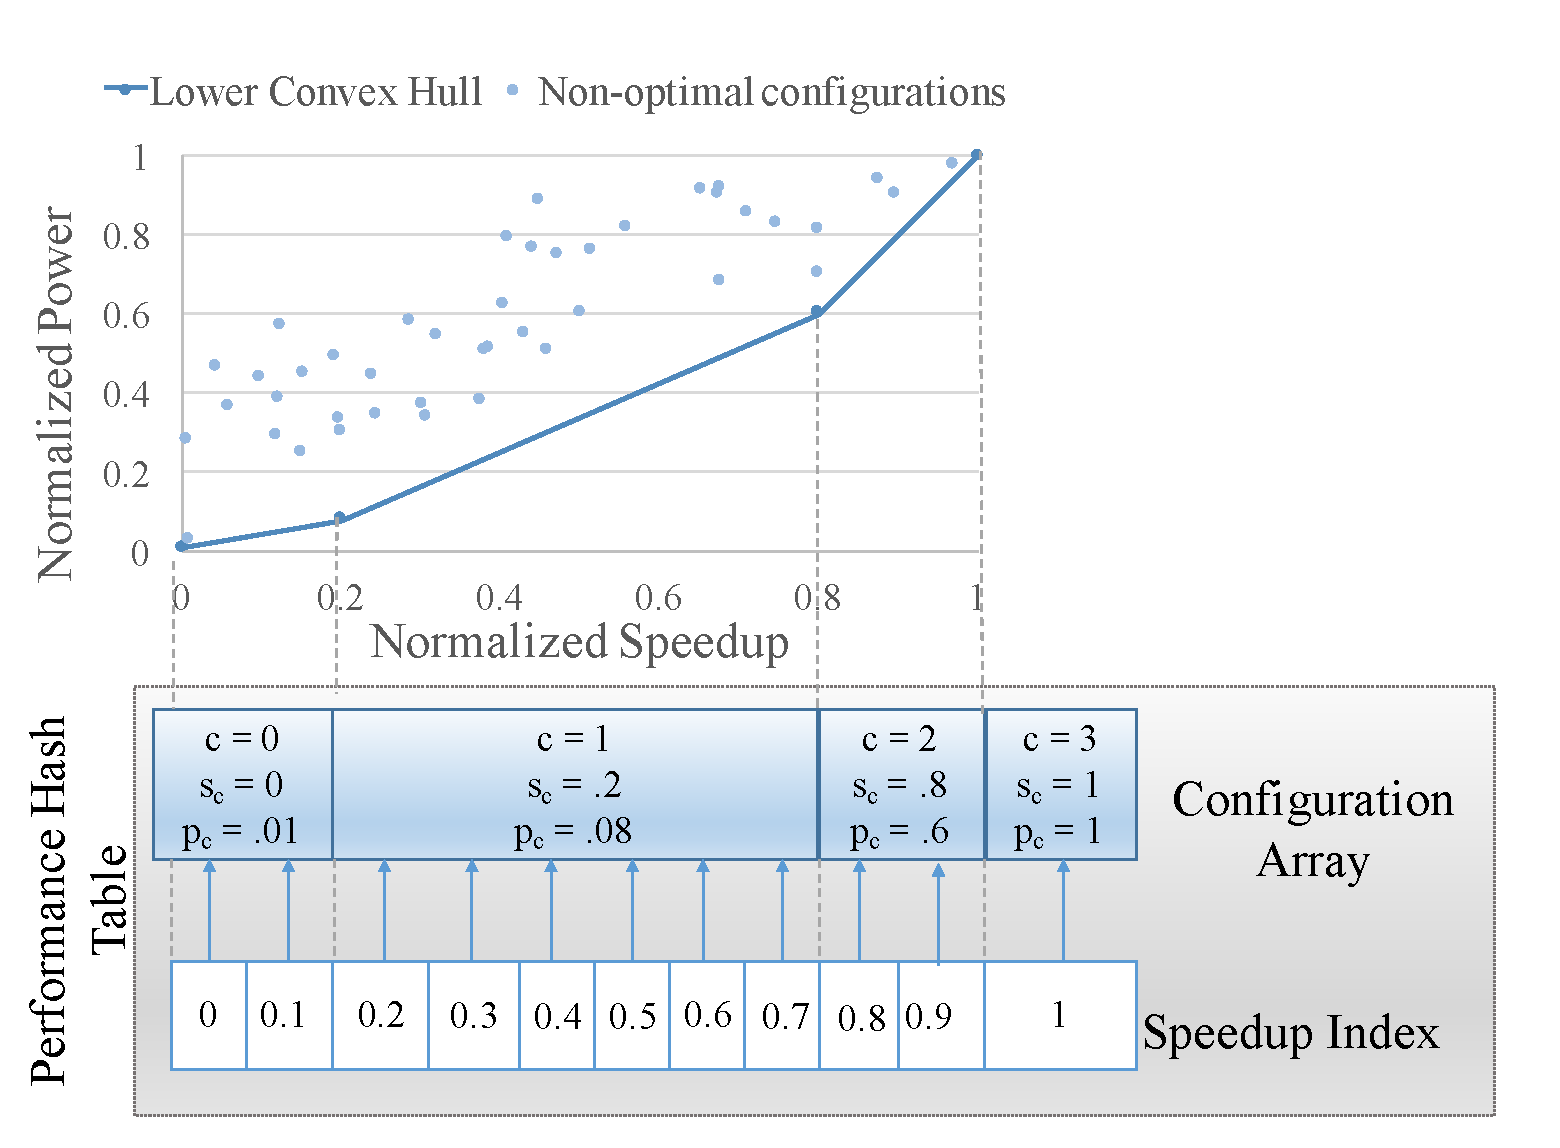
\includegraphics[width=\columnwidth]{figures/performance-hash-table.pdf}
\caption{Data structure to efficiently convert required speedup into a
  configuration.}
  \label{fig:pht}
\end{figure}

The PHT (illustrated in \figref{fig:pht}) only contains points on the
lower convex hull of the power/performance tradeoff space.  It
consists of two arrays: an array of pointers that point into a second
array, which stores the configurations on the convex hull sorted by
speedup.  Recall that speedups are computed relative to the base speed
which uses all resources.  We therefore know the largest speedup is 1,
so we need only concern ourselves with speedups less than 1.  The
first table, of pointers has a \emph{resolution} indicating how many
decimal points of precision it captures.  The example in
\figref{fig:pht} has a resolution of $0.1$.  Each pointer in the first
table points to the configuration in the second array that has the
largest speedup less than or equal to the index.

To use the table, the optimizer (\figref{fig:overview}) receives a
speedup $speedup(t)$ from the controller.  It converts this into two
configurations referred to as $hi$ and $lo$.  To find the $hi$
configuration, the translator clamps the desired speedup to the
largest index lower than $speedup(t)$ and then walks forward until it
finds the first configuration with a speedup higher than $speedup(t)$.
This configuration is $hi$.  To find the $lo$ configuration, the
translator clamps the desired speedup to the smallest index higher
than $speedup(t)$ and then walks backwards until it finds the
configuration with the largest speedup less than $speedup(t)$.

For example, consider the PHT in \figref{fig:pht} and an optimizer
meeting $speedup(t) = .65$.  To find $hi$, the optimizer indexes at .6
and walks up to find $c=2$ with $s_c=.8$, setting $hi = 2$.  To find
$lo$, the optimizer indexes the table at .7 and walks backward to find
$c=1$ with $s_c=.2$, setting $lo = 1$.

Finally, the optimizer sets $\tau_{hi}$ and $\tau_{lo}$ by solving the
following set of equations:
\begin{eqnarray}
  T &=& \tau_{hi} + \tau_{lo}    \label{eqn:s1} \\
  speedup(t) &=& \frac{s_{hi} \cdot \tau_{hi} + s_{lo} \cdot \tau_{lo}}{T} \label{eqn:s2}
\end{eqnarray}
In these equations, $speedup(t)$ is the speedup requested by the
controller and $s_c$ are speedups estimated by the learner.  By
solving \eqnsref{s1}{s2}, the optimizer has turned the controller's
speedup into a schedule of resource allocations using the models
provided by the HBM.

\PUNT{ Provided that the resolution is large enough to get a good
  spread of configurations to indices, the translator will always
  index the configuration array at most one entry from where it needs
  to be.  Thus, the entire translation process runs in constant time
  -- assuming that the learner is responsible for building the PHT
  once before passing it on to the translator.  This efficiency comes
  at a cost of memory usage -- many of the entries in the speedup
  index table will point to redundant locations in the configuration
  array.  We think that this is a reasonable tradeoff to make in
  practice as the code that runs on the mobile device must be fast or
  we risk wasting energy while trying to save energy.  In practice, we
  recommend a table of size 100 which provides a sufficient resolution
  and is not too wasteful of space.}


\subsection{Analysis}
%\subsubsection{Algorithmic Analysis}

\noindent \textbf{Control System Complexity} The GCS (see Algorithm
\ref{alg:gcs}) runs on the mobile or embedded device; each controller
invocation is $O(1)$ .  The only part that is not obviously constant
time is the PHT lookups.  Provided the PHT resolution is sufficiently
high to avoid collisions, then each PHT lookup requires constant time.
\begin{algorithm}[t]
\caption{Generalized control system}
\label{alg:gcs}
\begin{algorithmic}
\REQUIRE Initialize the controller with random configurations. Send power and performance samples to server and get performance hash table(PHT) from the server.
\WHILE{$True$}
    \STATE    Measure streaming application performance 
    \STATE    Compute required speedup (Equation \eqref{eqn:speedup})
    \STATE    Lookup $s_{hi}$ and $s_{lo}$ with PHT
    \STATE    Compute $\tau_{hi}$ and $\tau_{lo}$ (Equations \ref{eqn:s1} \& \ref{eqn:s2})
    \STATE    Configure to system to $hi$ $\&$ sleep $\tau_hi$.
    \STATE    Configure to $lo$ $\&$ sleep $\tau_lo$.
\ENDWHILE
\vskip -1.5em
\end{algorithmic}
\end{algorithm}


\noindent \textbf{Learning System Complexity} We run our learning
system on a remote server because the Hierarchical Bayesian Model
(HBM) is a relatively complex algorithm and it utilizes data from
other applications which can be stored in advance on the server
machines, allowing consolidation of data across similar devices.  The
time complexity for the HBM is $O(mn^3)$ where $m$ is the number of
applications and $n$ is the number of configurations.  Second step,
creating convex hull for the PHT takes $O(n log(n))$.

\subsection{Control Theoretic Formal Guarantees}
\label{sec:guarantees}
As mention above, the pole $\rho(t)$ is critical to connecting the control
system of Equation \ref{eqn:speedup} to the HBM of Equation
\ref{eq:HBN}.  In \SYSTEM{}, we know the model variance $\sigma$ from
the HBM so we use that information to derive a lower bound for the
pole which guarantees probabilistic convergence to the desired
performance. Specifically, we prove that with probability 99.7\% the
system will converge to the desired performance if the pole is set to,
$$\Floor{1- \Floor{max(\hat{s})/(min(\hat{s}) - 3\sigma)}_0}_0 \leq \rho(t)
< 1,$$ where $\Floor{x}_0 = \max(x,0)$ and $\hat{s}$ is the
estimated speedup. We include the proof of this claim in the appendix. In principle, users who need higher confidence
could set the scalar multiplier on $\sigma$ higher, using $6$ for
example provides a 99.99966\% probability of convergence.  

Thus we provide a lower-bound on the value of $\rho(t)$ required for a
user to be confident that CALOREE will converge to the desired
performance.  This value for the pole only considers performance,
and not energy efficiency.  In practice, we find that it is
often better to use a higher pole based on the \emph{uncertainty}
between the controller's observed energy efficiency and that predicted
by the model.  We follow prior work in quantifying uncertainty as
$\rho$ \cite{Tokic2010}:
\begin{equation}
  \begin{array}{rcl}
    \beta(t) &=&  \text{exp}{\left(- \left( \left|   \frac{\bar{s}(t)}{\bar{p}(t)}  -\frac{ \hat{s}(t)}{\hat{p}_(t)} \right| \right) /5\right)} \\
    \rho(t) &=& \frac{1-\beta(t)}{1+\beta(t)} 
  \end{array}
  \label{eqn:uncer}
\end{equation}
where $\bar{s}$ and $\bar{p}$ are the measured values of speedup and
power up and $\hat{s}$ and $\hat{p}$ are the estimated values from the
HBM.  This measure of uncertainty captures both power and performance.
We find that it is generally higher than the pole value given by our
lower bound, so in practice we set the pole dynamically to be the
higher of the two values and we allow the GCS to make spot updates to
the estimated speedup and power based on its observations.  
